\documentclass[preprint,12pt,authoryear]{elsarticle}
\usepackage[T1]{fontenc}
\usepackage{amsmath,amssymb,bm}
\usepackage{booktabs,multirow}
\usepackage{graphicx}
\usepackage{float}
\usepackage{algorithm}
\usepackage[noend]{algpseudocode}
\usepackage{xcolor}
\usepackage[hidelinks]{hyperref}
\usepackage{siunitx}
\graphicspath{{figures/}}
\newcommand{\CDvalue}{1.92}
\newcommand{\FriedmanChi}{364.8}
\newcommand{\FriedmanP}{4.4\times 10^{-73}}
\newcommand{\ShareAnimal}{63.5}
\newcommand{\ShareLocal}{13.4}
\newcommand{\ShareGravity}{12.9}
\newcommand{\ShareGlobal}{10.3}
\newcommand{\SharePlant}{36.5}
\newcommand{\CDGroups}{\{L-SHADE, APH, GA\}; \{APH, GA, PSO\}; \{DE, Hybrid-reinit, Hybrid, SDA\}; \{Hybrid-reinit, Hybrid, SDA, FPA\}; \{FPA, Random\}}
\newcommand{\SlopePre}{0.0044}
\newcommand{\SlopePost}{0.0376}
\newcommand{\SlopeRatio}{8.6}
\newcommand{\PageL}{2591}
\newcommand{\PageP}{3.3\times 10^{-12}}
\newcommand{\TauMonoRuns}{0}
\newcommand{\TauAdjMin}{0.38}
\newcommand{\TauFriedmanP}{6.1\times 10^{-6}}
\newcommand{\OneModelCI}{0.057}
\newcommand{\ValTestRho}{0.988}
\newcommand{\LRValSpec}{95.6}
\newcommand{\LRTestSpec}{58.1}
\newcommand{\LRValMCC}{0.898}
\newcommand{\EvalsReinit}{6794}
\newcommand{\EvalsTransfer}{6795}
\newcommand{\BootAphga}{+0.020 [+0.008, +0.032]}
\newcommand{\BootAphlShade}{-0.004 [-0.014, +0.006]}
\newcommand{\BootLShadega}{+0.024 [+0.012, +0.037]}
\newcommand{\BootHybridsda}{-0.013 [-0.029, +0.002]}
\newcommand{\BootHybridfpa}{+0.090 [+0.072, +0.106]}
\newcommand{\BootLogreglShade}{+0.050 [+0.004, +0.094]}
\newcommand{\BootMlpAdamaph}{+0.031 [-0.005, +0.068]}
\newcommand{\BootMemeticAphmlpAdam}{-0.013 [-0.031, +0.005]}
\newcommand{\MCCFpa}{0.260}
\newcommand{\ACCFpa}{64.9}
\newcommand{\MCCSda}{0.362}
\newcommand{\ACCSda}{70.7}
\newcommand{\MCCHybrid}{0.350}
\newcommand{\ACCHybrid}{70.3}
\newcommand{\MCCHybridReinit}{0.357}
\newcommand{\ACCHybridReinit}{70.6}
\newcommand{\MCCRandom}{0.178}
\newcommand{\ACCRandom}{61.5}
\newcommand{\MCCPso}{0.498}
\newcommand{\ACCPso}{77.1}
\newcommand{\MCCDe}{0.402}
\newcommand{\ACCDe}{72.6}
\newcommand{\MCCGa}{0.561}
\newcommand{\ACCGa}{79.8}
\newcommand{\MCCLShade}{0.585}
\newcommand{\ACCLShade}{80.9}
\newcommand{\MCCAph}{0.581}
\newcommand{\ACCAph}{80.7}
\newcommand{\MCCAdamOnly}{0.507}
\newcommand{\ACCAdamOnly}{77.4}
\newcommand{\MCCMemeticHybrid}{0.578}
\newcommand{\ACCMemeticHybrid}{80.2}
\newcommand{\MCCMemeticAph}{0.599}
\newcommand{\ACCMemeticAph}{81.1}
\newcommand{\MCCMajority}{0.000}
\newcommand{\ACCMajority}{62.5}
\newcommand{\MCCLogreg}{0.635}
\newcommand{\ACCLogreg}{82.7}
\newcommand{\MCCMlpSgd}{0.599}
\newcommand{\ACCMlpSgd}{80.9}
\newcommand{\MCCMlpAdam}{0.612}
\newcommand{\ACCMlpAdam}{81.5}
\newcommand{\WinFitHybridsda}{0}
\newcommand{\WinValHybridsda}{15}
\newcommand{\WinTestHybridsda}{22}
\newcommand{\WinFitHybridhybridReinit}{50}
\newcommand{\WinValHybridhybridReinit}{25}
\newcommand{\WinTestHybridhybridReinit}{26}
\newcommand{\WinFitHybridde}{32}
\newcommand{\WinValHybridde}{12}
\newcommand{\WinTestHybridde}{15}
\newcommand{\WinFitHybridfpa}{50}
\newcommand{\WinValHybridfpa}{47}
\newcommand{\WinTestHybridfpa}{43}
\newcommand{\WinFitSdafpa}{50}
\newcommand{\WinValSdafpa}{46}
\newcommand{\WinTestSdafpa}{36}
\newcommand{\WinFitAphlShade}{11}
\newcommand{\WinValAphlShade}{16}
\newcommand{\WinTestAphlShade}{19}
\newcommand{\WinFitAphga}{44}
\newcommand{\WinValAphga}{37}
\newcommand{\WinTestAphga}{37}
\newcommand{\FriedmanEightChi}{250.6}
\newcommand{\FriedmanEightP}{2.1\times 10^{-50}}
\newcommand{\FitHybrid}{0.70}
\newcommand{\FitSda}{0.46}
\newcommand{\FitDe}{0.82}
\newcommand{\FitAph}{0.176}
\newcommand{\FitLshade}{0.159}
\newcommand{\ValAph}{0.784}
\newcommand{\ValLshade}{0.797}
\newcommand{\ValHybrid}{0.516}
\newcommand{\ValSda}{0.548}
\newcommand{\SdaFpaDelta}{+0.103}
\newcommand{\SdaFpaP}{2.1\times 10^{-6}}
\newcommand{\AblUniformVsNoCx}{0.73}
\newcommand{\AblUniform}{-0.029}
\newcommand{\AblNoCx}{-0.031}
\newcommand{\AblPlant}{-0.199}
\newcommand{\OneModelLo}{0.06}
\newcommand{\OneModelHi}{0.08}
\newcommand{\NoOverlapN}{304}
\newcommand{\NoOverlapRho}{0.974}
\newcommand{\LRSensOverlap}{97.5}
\newcommand{\LRSensOther}{97.1}
\newcommand{\MlpSgdPcaAcc}{70.7}
\newcommand{\FTOffAcc}{89.0}
\newcommand{\FTOffSpec}{72.1}
\newcommand{\FTOffMin}{87.2}
\newcommand{\FTOffMax}{90.5}
\newcommand{\FTCvAcc}{97.4}
\newcommand{\FTCvSpec}{96.4}
\newcommand{\FTCvMcc}{0.935}
\newcommand{\FTCvAccTestFolder}{93.5}
\newcommand{\FTCvAccTrainFolder}{97.9}
\newcommand{\FTValAcc}{98.2}
\newcommand{\CvPatients}{3189}
\newcommand{\CvHeadRuns}{10}
\newcommand{\CvHeadN}{50}
\newcommand{\CvHeadHybrid}{97.1}
\newcommand{\CvHeadHybridBox}{96.8}
\newcommand{\CvHeadMin}{96.8}
\newcommand{\CvHeadMax}{97.6}
\newcommand{\CvHeadFpa}{96.9}
\newcommand{\CvHeadLshade}{97.4}
\newcommand{\CvHeadMlp}{97.5}
\newcommand{\CvHeadLogreg}{97.6}
\newcommand{\CvHeadFriedmanP}{1.9\times 10^{-14}}

\newcommand{\R}{\mathbb{R}}
\newcommand{\vecop}{\operatorname{vec}}
\newcommand{\clip}{\operatorname{clip}}
\renewcommand{\algorithmicrequire}{\textbf{Input:}}
\renewcommand{\algorithmicensure}{\textbf{Output:}}

\journal{a peer-reviewed journal}

\begin{document}
\begin{frontmatter}

\title{Do plant-inspired operators help to train a pneumonia classifier? A controlled benchmark and component analysis of a hybrid Flower Pollination--Seed Dispersal algorithm}

\author[iug]{Mona Alsbakhi}
\author[iug]{Mohammed Lubbad}
\author[iug]{Mohammed Alhanjouri\corref{cor1}}
\ead{mhanjouri@iugaza.edu.ps}
\cortext[cor1]{Corresponding author}
\affiliation[iug]{organization={Computer Engineering Department, Islamic University of Gaza},
            city={Gaza}, country={Palestine}}

\begin{abstract}
Hybrids of nature-inspired metaheuristics are frequently proposed for training neural networks in medical imaging, usually on the strength of a single favourable comparison. We examine one such design, a sequential hybrid of the Flower Pollination Algorithm (FPA) and a seed-dispersal algorithm (SDA), on the paediatric chest X-ray pneumonia dataset under a controlled protocol: a patient-grouped validation split, the official test folder (624 images), a common budget of 6,795 fitness evaluations for the gradient-free optimisers, 50 paired runs in the main benchmark and non-parametric statistics on three endpoints (training fitness, validation MCC and test MCC). On frozen ResNet-50 features with a 2048--16--2 classifier head the hybrid reaches a test MCC of \MCCHybrid{} (accuracy \ACCHybrid\%). It is better than FPA (\MCCFpa) and random search on every endpoint; it reaches a worse training fitness than SDA alone in all 50 runs, with a similar test MCC (\MCCSda); and it is below GA (\MCCGa), PSO (\MCCPso) and L-SHADE (\MCCLShade). Lengthening the FPA phase gives a decreasing trend (Page's test $p=\PageP$). A redesigned hybrid that adds the FPA and SDA operators to a success-history differential-evolution framework (APH, designed after these results were known) reaches \MCCAph{}, but L-SHADE without those operators attains a lower training fitness in most runs, and APH restricted to the plant-inspired operators falls back to 0.382. On the original 138,530-dimensional PCA pipeline with standardised inputs, none of the seven gradient-free optimisers tested exceeds chance level. Gradient-trained classifiers are best on frozen features (logistic regression \MCCLogreg). Fine-tuning the network by backpropagation raises accuracy to \FTOffAcc\% on the official test folder and \FTCvAcc\% under patient-grouped five-fold cross-validation, and on the fine-tuned features every optimiser, including the original hybrid (\CvHeadHybrid\%), lies between \CvHeadMin\% and \CvHeadMax\%. On this task the representation, not the choice of optimiser, determines accuracy, and the plant-inspired operators bring no benefit over established components. Code, configurations and per-run outputs are released.
\end{abstract}

\begin{keyword}
Flower pollination algorithm \sep Seed dispersal \sep Hybrid metaheuristics \sep Neuroevolution \sep Benchmarking \sep Ablation \sep Pneumonia detection \sep Chest X-ray
\end{keyword}
\end{frontmatter}

%% ===========================================================================
\section{Introduction}\label{sec:intro}

Deep networks trained by gradient descent are the standard tool for medical image classification \citep{lecun2015deep,litjens2017survey}, and pneumonia detection on chest radiographs is a well-studied instance \citep{kermany2018,rajpurkar2017chexnet}. In parallel, a large literature trains or tunes networks with population-based metaheuristics \citep{ojha2017metaheuristic,stanley2019neuroevolution}, motivated by the non-convexity of the loss surface and by settings in which gradients are unavailable. Many recent contributions are hybrids of two metaphor-based algorithms evaluated on a single dataset against their own components. The evolutionary-computation community has repeatedly cautioned that such designs often recombine known operators under new names and are rarely compared against established methods under equal budgets \citep{sorensen2015metaphor,aranha2022callforaction,camacho2023exposing}.

This study started from our own unpublished draft, which proposed a sequential hybrid of the Flower Pollination Algorithm \citep{yang2012fpa} and a seed-dispersal algorithm (FPA--SDA) for training a multilayer perceptron on PCA-reduced chest radiographs and presented it as the most accurate method tested; its notebook is included in the repository as the ``original implementation''. Re-examining that claim with a reproducible pipeline changed the conclusion: under equal budgets and paired statistics the hybrid is neither better than its second component nor competitive with standard metaheuristics or with gradient training. Rather than tune the method until it appears superior, this paper reports the controlled comparison and asks which components, if any, make a hybrid of this kind work.

The contributions are:
\begin{itemize}
\item A reproducible benchmark of FPA, SDA and their sequential hybrid against GA, PSO, DE, L-SHADE, random search, evolution strategies, zeroth-order SGD and gradient-trained classifiers, on the official test split with a patient-grouped validation split, equal evaluation budgets and 50 paired runs (Sections~\ref{sec:methods}--\ref{sec:results}).
\item A statistical analysis on three endpoints---training fitness, validation MCC and test MCC---with Friedman and Nemenyi tests, Holm-adjusted Wilcoxon tests, effect sizes and test-image bootstrap intervals, and a sensitivity study of the transition point $\tau$ (Section~\ref{sec:stats}).
\item A redesigned hybrid (APH) that selects FPA and SDA operators adaptively inside a success-history DE framework, and an ablation showing that its gains depend on established DE components, while adding the plant-inspired operators to L-SHADE slightly worsens optimisation on this task (Section~\ref{sec:redesign}).
\item Evidence on the original high-dimensional pipeline ($D=138{,}530$), on memetic variants that combine the hybrid with Adam, and on fine-tuned features under patient-grouped cross-validation, showing that the representation rather than the optimiser determines accuracy (Sections~\ref{sec:pca}, \ref{sec:finetune} and \ref{sec:discussion}).
\end{itemize}

%% ===========================================================================
\section{Related work}\label{sec:related}

\paragraph{Metaheuristic training of neural networks} Population-based optimisation of network weights has been studied for over three decades; \citet{ojha2017metaheuristic} review its use for feed-forward networks and \citet{stanley2019neuroevolution} survey neuroevolution more broadly. Two strands are relevant here. Large-scale gradient-free methods scale by exploiting structure: limited-memory matrix adaptation \citep{loshchilov2019lmmaes}, evolution strategies with antithetic sampling and rank shaping \citep{salimans2017es}, which have recently been applied to full-parameter fine-tuning of billion-parameter language models \citep{qiu2025esllm}, and zeroth-order SGD with two-point simultaneous-perturbation estimates \citep{spall1992spsa,malladi2023mezo}. Differential evolution \citep{storn1997de} with success-history parameter adaptation \citep{zhang2009jade,tanabe2013shade} and linear population-size reduction \citep{tanabe2014lshade} remains the reference design for bound-constrained black-box optimisation; strategy adaptation over several mutation operators was introduced by SaDE \citep{qin2009sade} and studied with probability matching and adaptive pursuit by \citet{gong2011strategy}. For network training specifically, \citet{piotrowski2014stagnation} showed that DE variants are prone to stagnation. Genetic algorithms have been shown to train deep networks competitively in reinforcement learning \citep{such2017deep}, and NeuroEvoBench provides standardised comparisons of evolutionary optimisers for deep learning \citep{lange2023neuroevobench}.

\paragraph{Plant-inspired algorithms} FPA \citep{yang2012fpa} alternates Lévy-flight moves towards the best solution with differential local moves; numerous variants adjust the switch probability or step sizes \citep{abdelbasset2019fpareview}, and hybrids with differential evolution have been proposed \citep{song2024defpa}. Seed-dispersal mechanisms underlie the seed-based plant propagation algorithm \citep{sulaiman2015sbppa} and the Fertile Field Algorithm \citep{mohammadi2020ffa}. In medical applications FPA has been used to weight CNN ensembles \citep{zhou2025fpaensemble} and to train neuro-fuzzy predictors \citep{kaya2024fpaanfis}; metaheuristic feature selection and weight training on chest radiographs have also been reported \citep{elkenawy2021,almutairi2024}.

\paragraph{Evaluation practice} Comparisons of stochastic optimisers require multiple independent runs, equal budgets, appropriately tuned competitors and non-parametric tests \citep{derrac2011tutorial,demsar2006,eiben2011parameter}. The no-free-lunch theorems \citep{wolpert1997nfl} imply that any claimed advantage is problem-specific and must be demonstrated against strong baselines on the problem at hand. The critique of metaphor-based metaheuristics \citep{sorensen2015metaphor,camacho2023exposing} adds that new algorithms should be described in standard terminology and their components evaluated separately \citep{lones2020metaphors}. Component-level analyses have shown that cuckoo search, another Lévy-flight method, adds no new ideas \citep{camacho2022cuckoo}, that several metaheuristics improve when components are removed \citep{piotrowski2018simplified}, and that the chimp optimisation algorithm is structurally biased \citep{deng2024chimp}. Section~\ref{sec:redesign} takes this approach.

Table~\ref{tab:taxonomy} positions this study relative to these strands.

\begin{table}[!t]
\centering
\caption{Positioning of this study.}
\label{tab:taxonomy}
\footnotesize
\begin{tabular}{p{3.0cm}p{3.6cm}p{5.2cm}}
\toprule
Strand & Representative work & Gap addressed here \\
\midrule
Plant-inspired optimisers & \citet{yang2012fpa}; \citet{abdelbasset2019fpareview}; \citet{sulaiman2015sbppa} & Operators evaluated in isolation against DE-type components (ablation) \\
FPA in medical AI & \citet{zhou2025fpaensemble}; \citet{kaya2024fpaanfis} & Weight training under equal budgets, paired runs, official test split \\
Adaptive DE & \citet{zhang2009jade}; \citet{tanabe2013shade,tanabe2014lshade} & Used as strong baseline and as host framework for APH \\
Large-scale gradient-free & \citet{salimans2017es}; \citet{malladi2023mezo}; \citet{qiu2025esllm} & Included as cross-field baselines \\
Evaluation methodology & \citet{derrac2011tutorial}; \citet{demsar2006}; \citet{sorensen2015metaphor} & Applied throughout; component-level conclusions \\
\bottomrule
\end{tabular}
\end{table}

%% ===========================================================================
\section{Methods}\label{sec:methods}

\subsection{Data and splits}
We use the Kermany paediatric chest X-ray dataset \citep{kermany2018} in its Kaggle distribution \citep{kaggle2018cxr}: 5,856 images (1,583 normal, 4,273 pneumonia). The official \emph{test} folder (234 normal, 390 pneumonia) is held out and used once per trained model. The official 16-image validation folder is merged into the training folder, which is then split by patient into an optimisation subset (4,186 images; 1,079/3,107) and a validation subset (1,046; 270/776) with a stratified group split, so that no patient contributes to both. Patient identifiers are parsed from file names. All fitness evaluations use the optimisation subset only; the validation subset is used for reporting and the test set for final evaluation. Of the 431 patient identifiers in the test folder, 170 also occur in the training folder; since no test image has a cosine similarity above 0.931 to any training image in the ResNet-50 feature space, these are probably independent numberings, but cross-split patient overlap cannot be excluded from file names alone. The test folder contains six near-identical image pairs (cosine similarity $>0.99$), which are kept to preserve the official split.

\subsection{Feature pipelines}
\emph{CNN features (main experiments).} Each image is converted to three identical channels, resized to $224\times224$ and passed through an ImageNet-pretrained ResNet-50 \citep{he2016resnet,deng2009imagenet} with frozen weights; the 2048-dimensional global-average-pooled output is standardised with statistics of the optimisation subset.
\emph{PCA features (original pipeline).} Images are resized to $150\times150$, scaled to $[0,1]$, flattened ($22{,}500$ values) and projected onto the first 1,000 principal components of the optimisation subset, either as raw scores (as in the original implementation) or standardised.

\subsection{Network and solution encoding}
A fully connected network with ReLU hidden layers and a two-unit softmax output maps a feature vector $\mathbf{a}^{(0)}\in\R^{d}$ to class probabilities. For layers $l=1,\dots,L$ with weights $W^{(l)}\in\R^{n_{l-1}\times n_l}$ and biases $\mathbf{b}^{(l)}\in\R^{n_l}$, every candidate solution is the concatenation
\begin{equation}
\begin{gathered}
\mathbf{x}=\left[\vecop(W^{(1)})^{\top},\dots,\vecop(W^{(L)})^{\top},(\mathbf{b}^{(1)})^{\top},\dots,(\mathbf{b}^{(L)})^{\top}\right]^{\top}\in\R^{D},\\
D=\sum_{l=1}^{L}n_l\,(n_{l-1}+1),
\end{gathered}
\label{eq:encoding}
\end{equation}
with all weight matrices first and all bias vectors last, exactly as in the implementation. For the CNN head ($2048$--$16$--$2$, $L=2$) $D=32{,}818$; for the original PCA network ($1000$--$128$--$64$--$32$--$2$, $L=4$) $D=128{,}128+8{,}256+2{,}080+66=138{,}530$. All search methods operate in the box $[lb,ub]^D=[-1,1]^D$ and initialise uniformly within it.

\subsection{Fitness function}
Given $m$ optimisation images with labels $y_i\in\{0,1\}$ and predicted class probabilities $\hat p_{i,c}(\mathbf{x})$, the fitness to be minimised is the class-weighted cross-entropy plus an $L_2$ penalty on the weights,
\begin{align}
f(\mathbf{x}) &= \mathcal{L}_{\mathrm{CE}}(\mathbf{x})+\mathcal{L}_{L_2}(\mathbf{x}),\label{eq:fitness}\\
\mathcal{L}_{\mathrm{CE}}(\mathbf{x}) &= -\frac{1}{m}\sum_{i=1}^{m} w_{y_i}\log \hat p_{i,y_i}(\mathbf{x}),\qquad w_c=\frac{m}{2\,m_c},\label{eq:ce}\\
\mathcal{L}_{L_2}(\mathbf{x}) &= \frac{\lambda}{2m}\sum_{l=1}^{L}\sum_{j,k}\bigl(W^{(l)}_{jk}\bigr)^2,\qquad \lambda=10^{-3},\label{eq:l2}
\end{align}
where $m_c$ is the number of class-$c$ images. Eq.~\eqref{eq:ce} is the two-class softmax form of binary cross-entropy with balanced class weights; log-probabilities are computed with a numerically stable log-sum-exp.

\subsection{Flower Pollination Algorithm}
At iteration $t$, flower $i$ produces a candidate $\mathbf{v}_i$ by global pollination with probability $p=0.8$ and by local pollination otherwise:
\begin{align}
\mathbf{v}_i &= \mathbf{x}_i^{(t)}+\gamma\,\mathbf{L}\odot\bigl(\mathbf{g}^{*}-\mathbf{x}_i^{(t)}\bigr),\label{eq:fpa_global}\\
\mathbf{v}_i &= \mathbf{x}_i^{(t)}+\bm{\epsilon}\odot\bigl(\mathbf{x}_j^{(t)}-\mathbf{x}_k^{(t)}\bigr),\qquad \bm{\epsilon}\sim U(0,1)^D,\ j\neq k,\label{eq:fpa_local}
\end{align}
where $\mathbf{g}^{*}$ is the best solution found so far and $\odot$ denotes element-wise multiplication. Eq.~\eqref{eq:fpa_global} uses the direction from $\mathbf{x}_i$ to $\mathbf{g}^{*}$, as in Yang's pseudocode \citep{yang2012fpa}; because the Lévy step is symmetric, each coordinate moves towards or away from $\mathbf{g}^{*}$ with equal probability. The implementation used throughout uses $\gamma=1$. Each component of the Lévy step $\mathbf{L}\in\R^D$ is drawn with Mantegna's algorithm \citep{mantegna1994} with $\beta=1.5$:
\begin{equation}
\begin{gathered}
L_d=\frac{u_d}{|v_d|^{1/\beta}},\quad u_d\sim\mathcal{N}(0,\sigma_u^2),\ v_d\sim\mathcal{N}(0,1),\\[2pt]
\sigma_u=\left[\frac{\Gamma(1+\beta)\sin(\pi\beta/2)}{\Gamma\!\left(\frac{1+\beta}{2}\right)\beta\,2^{(\beta-1)/2}}\right]^{1/\beta}.
\end{gathered}
\label{eq:mantegna}
\end{equation}
Candidates are clipped to $[lb,ub]$ and replace $\mathbf{x}_i$ only if strictly better (greedy, in-place selection); $\mathbf{g}^{*}$ is updated immediately.

\subsection{Seed-dispersal algorithm}
Each seed applies one of three dispersal operators, chosen with probabilities $(P_{\mathrm{wind}},P_{\mathrm{animal}},P_{\mathrm{gravity}})=(0.70,0.15,0.15)$:
\begin{align}
\text{wind:}\quad & \mathbf{v}_i=\mathbf{x}_i^{(t)}+\mathbf{L}\odot\bigl(\mathbf{g}^{*}-\mathbf{x}_i^{(t)}\bigr),\label{eq:wind}\\
\text{animal:}\quad & \mathbf{v}_i=\mathbf{x}_i^{(t)}+\bm{\epsilon}\odot\bigl(\mathbf{x}_r^{(t)}-\mathbf{x}_i^{(t)}\bigr),\qquad \bm{\epsilon}\sim U(0,1)^D,\ r\sim U\{1,\dots,n\},\label{eq:animal}\\
\text{gravity:}\quad & \mathbf{v}_i=\mathbf{x}_i^{(t)}+\mathbf{s},\qquad \mathbf{s}\sim U(-0.1,0.1)^D,\label{eq:gravity}
\end{align}
followed by clipping and the same strictly-better greedy selection. With $\gamma=1$ the FPA global operator \eqref{eq:fpa_global} and the SDA wind operator \eqref{eq:wind} are identical; FPA and SDA therefore differ only in their remaining operators and in the probability of the Lévy move ($0.8$ versus $0.7$). Our original draft attributed these operators to two prior publications that we could not verify; the operators are therefore documented here exactly as implemented, and seed-dispersal-inspired optimisers in the literature are cited for context only \citep{sulaiman2015sbppa,mohammadi2020ffa}.

\subsection{Sequential hybrid FPA--SDA}\label{sec:hybrid}
The hybrid runs FPA for $\tau$ iterations and SDA for the remaining $T-\tau$ iterations ($T=150$, $\tau=75$, $n=45$). Let $\mathbf{x}^{*}_{\mathrm{FPA}}$ denote the best solution after phase 1 and $\{\mathbf{x}_i^{(\tau)}\}$ the phase-1 population. Two transition operators are studied.

\emph{Transfer (original implementation).} The SDA phase starts from the final FPA population unchanged:
\begin{equation}
\mathbf{x}_i^{(\tau^{+})}=\mathbf{x}_i^{(\tau)},\qquad i=1,\dots,n.
\label{eq:transfer}
\end{equation}

\emph{Re-initialisation around the elite.} The elite is kept and the other $n-1$ seeds are resampled around it with controlled diversity:
\begin{equation}
\begin{gathered}
\mathbf{x}_1^{(\tau^{+})}=\mathbf{x}^{*}_{\mathrm{FPA}},\\
\mathbf{x}_i^{(\tau^{+})}=\clip\!\Bigl(\mathbf{x}^{*}_{\mathrm{FPA}}+\sigma_{\mathrm{init}}\,\mathbf{z}_i,\;lb,\;ub\Bigr),\quad \mathbf{z}_i\sim\mathcal{N}(\mathbf{0},\mathbf{I}_D),\quad i=2,\dots,n,
\end{gathered}
\label{eq:reinit}
\end{equation}
with $\sigma_{\mathrm{init}}=0.05\,(ub-lb)=0.1$. The $n-1$ new seeds are evaluated and the SDA phase is shortened by one iteration, so the transfer variant uses $n(T+1)=6{,}795$ evaluations and the re-initialisation variant \EvalsReinit{} (the elite is not re-evaluated). Our original draft described Eq.~\eqref{eq:reinit} while its code implemented Eq.~\eqref{eq:transfer}; both are therefore reported. Algorithm~\ref{alg:hybrid} gives the complete procedure.

\begin{algorithm}[!t]
\caption{Sequential hybrid FPA--SDA for network-weight optimisation}\label{alg:hybrid}
\footnotesize
\begin{algorithmic}[1]
\Require features $X\in\R^{m\times d}$ (PCA or CNN), labels $\mathbf{y}$; layer sizes $(n_0{=}d,\dots,n_L{=}2)$;\Statex \hspace{\algorithmicindent} $n{=}45$, $T{=}150$, $\tau{=}75$, $p{=}0.8$, $(P_{\mathrm{wind}},P_{\mathrm{animal}},P_{\mathrm{gravity}}){=}(0.70,0.15,0.15)$;\Statex \hspace{\algorithmicindent} $[lb,ub]{=}[-1,1]$, $\lambda{=}10^{-3}$, $\sigma_{\mathrm{init}}{=}0.1$, mode $\in\{\textsc{transfer},\textsc{reinit}\}$
\Ensure network parameters $\mathbf{x}^{*}\in\R^{D}$, $D$ from Eq.~\eqref{eq:encoding}
\State \textbf{for} $i=1..n$: $\mathbf{x}_i\sim U(lb,ub)^D$; decode $\mathbf{x}_i\mapsto\{W^{(l)},\mathbf{b}^{(l)}\}$; $f_i\gets f(\mathbf{x}_i)$ \Comment{Eqs.~\eqref{eq:encoding}--\eqref{eq:l2}}
\State $\mathbf{g}^{*}\gets\arg\min_i f_i$
\For{$t=1$ \textbf{to} $\tau$} \Comment{Phase 1: FPA}
  \For{$i=1$ \textbf{to} $n$}
    \If{$U(0,1)<p$} \State $\mathbf{v}\gets$ global pollination, Eqs.~\eqref{eq:fpa_global}--\eqref{eq:mantegna}
    \Else \State $\mathbf{v}\gets$ local pollination, Eq.~\eqref{eq:fpa_local}
    \EndIf
    \State $\mathbf{v}\gets\clip(\mathbf{v},lb,ub)$; \textbf{if} $f(\mathbf{v})< f_i$ \textbf{then} $(\mathbf{x}_i,f_i)\gets(\mathbf{v},f(\mathbf{v}))$; update $\mathbf{g}^{*}$
  \EndFor
\EndFor
\State $T_2\gets T-\tau$
\If{mode $=\textsc{reinit}$} \Comment{Phase transition, Eq.~\eqref{eq:reinit}}
  \State $\mathbf{x}_1\gets\mathbf{g}^{*}$; \textbf{for} $i=2..n$: $\mathbf{x}_i\gets\clip(\mathbf{g}^{*}+\sigma_{\mathrm{init}}\mathbf{z}_i,lb,ub)$, $f_i\gets f(\mathbf{x}_i)$; \ $T_2\gets T_2-1$
\EndIf \Comment{mode \textsc{transfer}: population kept, Eq.~\eqref{eq:transfer}}
\For{$t=1$ \textbf{to} $T_2$} \Comment{Phase 2: SDA}
  \For{$i=1$ \textbf{to} $n$}
    \State $r\sim U(0,1)$
    \If{$r<0.70$} \State $\mathbf{v}\gets$ wind dispersal, Eq.~\eqref{eq:wind}
    \ElsIf{$r<0.85$} \State $\mathbf{v}\gets$ gravity dispersal, Eq.~\eqref{eq:gravity}
    \Else \State $\mathbf{v}\gets$ animal dispersal, Eq.~\eqref{eq:animal}
    \EndIf
    \State $\mathbf{v}\gets\clip(\mathbf{v},lb,ub)$; \textbf{if} $f(\mathbf{v})< f_i$ \textbf{then} $(\mathbf{x}_i,f_i)\gets(\mathbf{v},f(\mathbf{v}))$; update $\mathbf{g}^{*}$
  \EndFor
\EndFor
\State \Return $\mathbf{x}^{*}\gets\mathbf{g}^{*}$
\end{algorithmic}
\end{algorithm}

\subsection{Redesigned hybrid: Adaptive Plant Hybrid (APH)}\label{sec:aph}
The benchmark (Section~\ref{sec:results}) suggests three weaknesses of the sequential design: a fixed, harmful phase schedule; operators that perturb all $D$ coordinates at once; and fixed parameters. APH replaces phase-level by operator-level hybridisation. In each generation every individual draws one of four operators,
\begin{align*}
\text{O1 (FPA global)}:\ & \mathbf{v}=\mathbf{x}_i+F\,\clip(\mathbf{L},-3,3)\odot(\mathbf{g}^{*}-\mathbf{x}_i)\\
\text{O2 (FPA local)}:\ & \mathbf{v}=\mathbf{x}_i+F\,(\mathbf{x}_j-\mathbf{x}_k)\\
\text{O3 (SDA animal, current-to-}p\text{best)}:\ & \mathbf{v}=\mathbf{x}_i+F\,(\mathbf{x}_{p\mathrm{best}}-\mathbf{x}_i)+F\,(\mathbf{x}_{r_1}-\tilde{\mathbf{x}}_{r_2})\\
\text{O4 (SDA gravity)}:\ & \mathbf{v}=\mathbf{x}_i+F\,\mathbf{s}\odot\mathbf{z},\quad \mathbf{z}\sim\mathcal{N}(\mathbf{0},\mathbf{I}),
\end{align*}
where $\mathbf{x}_{p\mathrm{best}}$ is drawn from the best $11\%$, $\tilde{\mathbf{x}}_{r_2}$ from the population plus an archive of replaced parents, and $\mathbf{s}$ is the per-coordinate population standard deviation. The candidate is combined with $\mathbf{x}_i$ by binomial crossover with rate $CR$, so only part of the weight vector changes. $F$ and $CR$ are sampled from success-history memories (Cauchy and normal, respectively, $H=6$) updated with weighted Lehmer and arithmetic means \citep{tanabe2013shade}; operator probabilities follow probability matching on relative improvement with a floor of $0.05$ \citep{thierens2005aos}; the population shrinks linearly from 45 to 4 \citep{tanabe2014lshade}. O3 is the current-to-$p$best/1 mutation of JADE \citep{zhang2009jade}; the ablation in Section~\ref{sec:redesign} isolates its contribution.

\subsection{Comparators}
All gradient-free methods receive $n(T+1)=6{,}795$ fitness evaluations (\EvalsReinit{} for the re-initialisation variant of the hybrid), start from the same uniform population (shared random seed per run) and use the same bounds; parameters are listed in Table~\ref{tab:params}:
random search (uniform resampling with per-slot replacement);
GA (steady-state, binary tournament, BLX-$\alpha$ crossover with $\alpha=0.5$, Gaussian mutation, worst replacement);
PSO with constriction coefficients \citep{kennedy1995pso,clerc2002constriction};
DE/rand/1/bin with $F=0.5$, $CR=0.9$ \citep{storn1997de};
L-SHADE \citep{tanabe2014lshade};
OpenAI-ES with antithetic sampling, centred-rank shaping and Adam ($\sigma=0.02$, learning rate $0.01$) \citep{salimans2017es};
and ZO-SGD with two-point SPSA estimates \citep{spall1992spsa,malladi2023mezo}.
Memetic variants spend half the budget on the hybrid or APH and then apply 300 full-batch Adam steps \citep{kingma2015adam} (learning rate $10^{-3}$) using exact gradients of Eq.~\eqref{eq:fitness}; the Adam-only control applies the same steps to the best of the 45 uniform initial solutions.
Gradient-trained references are logistic regression and an MLP of the same architecture trained by backpropagation with Adam or SGD with momentum and early stopping \citep{pedregosa2011sklearn}, plus the majority-class predictor. The finite-difference ``SGD'' baseline of our original draft is not used: it estimated gradients on 1,000 random coordinates per step and is not representative of gradient training.

\subsection{Fine-tuning, cross-validation and head training on fine-tuned features}\label{sec:ftmethods}
To separate the effect of the representation from that of the optimiser, the ResNet-50 was also fine-tuned end to end by backpropagation: AdamW \citep{loshchilov2019adamw} with a one-cycle learning-rate schedule (peak $3\times10^{-4}$), weight decay $10^{-4}$, 12 epochs, batch size 64, class-weighted cross-entropy and mixed precision; images are stored at $256\times256$ and augmented to $224\times224$ by random scaling (0.85--1), rotation ($\pm10^{\circ}$), translation and brightness and contrast jitter. The epoch is selected by validation MCC and the held-out data are evaluated once per model. Two protocols are used: (i) the official split, with five seeds; and (ii) patient-grouped five-fold cross-validation over all 5,856 images (\CvPatients{} patient identifiers; identifiers that occur in both official folders are kept in one fold), with an inner patient-grouped split of the training folds (one eighth) for epoch selection, and three seeds. These hyperparameters were fixed before the cross-validation and were not tuned on it. Models were trained on an NVIDIA A100 with PyTorch 2.14.1.

For the seed-0 model of each fold, the 2048-dimensional penultimate features were extracted and the 2048--16--2 head was trained by each optimiser (\CvHeadRuns{} runs per fold, new seeds). In these runs the gradient-free optimisers search a Glorot-scaled space, $\bm\theta=\mathbf{s}\odot\mathbf{z}$ with $\mathbf{z}\in[-1,1]^D$ and $\mathbf{s}$ equal to twice the Glorot-uniform limit of each layer \citep{glorot2010}; the hybrid is also run in the original $[-1,1]^D$ box.

\subsection{Protocol and statistical analysis}\label{sec:protocol}
Each method is run 50 times (20 for the $\tau$ study and the ablation, 10 for the PCA pipeline) with run-indexed seeds shared across methods, giving paired samples. Three endpoints are analysed. Optimisers are compared on the final training fitness, which is the quantity they minimise, and on validation MCC; classifiers are compared on the test set by accuracy, balanced accuracy, sensitivity, specificity and Matthews correlation coefficient (MCC), all computed from one confusion matrix at a threshold of 0.5, and by ROC AUC computed from the predicted probabilities. Methods are compared with the Friedman test \citep{friedman1937} followed by the Nemenyi post-hoc test with critical difference $\mathrm{CD}=q_{\alpha}\sqrt{k(k+1)/(6N)}$ \citep{demsar2006}, and pairwise with the Wilcoxon signed-rank test \citep{wilcoxon1945} with Holm correction \citep{holm1979}; effect sizes are reported as the Vargha--Delaney $\hat A$ statistic \citep{vargha2000}. Two effect measures are reported: $\bar\Delta$, the difference of means, and $\tilde\Delta$, the median of paired differences. A monotone trend over the transition point is tested with Page's $L$ test \citep{page1963trend}. Because all runs are evaluated on the same 624 test images, $p$-values across seeds do not capture test-set sampling uncertainty; we therefore also resample test images with replacement (2,000 bootstrap samples, seeds held fixed) and report 95\% intervals for key differences, recomputed from the stored predictions. The protocol follows \citet{derrac2011tutorial}.

\emph{Design history.} The experiments were not all planned in advance, and the order matters for interpretation. (i) The original PCA pipeline was run first; after a one-run pilot showed the gradient-free optimisers at chance level, its run count was fixed at 10. (ii) The CNN-feature task was then introduced, with eight gradient-free optimisers (FPA, SDA, the two hybrids, random search, PSO, DE, GA) and the gradient-trained references, 50 runs each, followed by the $\tau$ study. (iii) APH, the memetic variants, and the additional baselines L-SHADE, OpenAI-ES and ZO-SGD were added afterwards, with knowledge of the earlier results including test-set metrics; a five-run pilot of these methods used seeds 0--4, and those runs are part of the 50 reported. (iv) The analysis of training fitness and validation MCC, the fine-tuning experiments and the Glorot-scaled search space (Section~\ref{sec:ftmethods}) were added after independent review of a draft; these use seeds not used before, and their settings were fixed before they were run. Results for the methods in (iii) and (iv) are exploratory; the Friedman test over the eight optimisers of step (ii) alone gives $\chi^2_F=\FriedmanEightChi$, $p=\FriedmanEightP$.

\subsection{Implementation and reproducibility}
All methods are implemented in Python 3.13 with NumPy 2.5, SciPy 1.18 and scikit-learn 1.9; Frozen ResNet-50 features are extracted with PyTorch 2.15.0 and torchvision 0.29.2 (CPU) using the \texttt{IMAGENET1K\_V2} weights. Each (method, run) pair writes a JSON file containing the configuration, seed, convergence history, evaluation count, run time, validation and test metrics and the test-set probabilities; every table and figure in this paper is generated from these files by a single script. Run times were measured on a 4-core cloud CPU with four runs executing concurrently, one thread each, and are indicative only. Code, configurations and all per-run outputs are available at \citet{alsbakhi2026code}.

%% ===========================================================================
\section{Results}\label{sec:results}

\subsection{Original pipeline: PCA features, $D=138{,}530$}\label{sec:pca}
Table~\ref{tab:pca} reports the original high-dimensional setting. With raw PCA scores, as in the original implementation, SDA alone reaches 68.5\% accuracy, the hybrid 60.4\% and FPA 56.5\%; the hybrid is therefore not the most accurate method in the original setting either. With standardised scores all seven gradient-free optimisers run on this pipeline (FPA, SDA, the two hybrids, PSO, DE and GA) and random search are at chance level (AUC 0.50--0.52), and their median best training fitness (e.g.\ SDA 0.82, hybrid 1.19) remains above $\ln 2\approx0.69$, the loss of a constant predictor; logistic regression and the backpropagation-trained MLPs reach \MlpSgdPcaAcc--74.4\%. L-SHADE, APH, OpenAI-ES and ZO-SGD were not run on this pipeline. Because SDA reaches MCC 0.347 at the same dimension with raw scores, dimension alone does not explain the failure; input scaling, the search box and the budget may all contribute, but none of them was varied here. The remaining experiments use the CNN head.

\begin{table}[!t]
\centering
\caption{Original pipeline: PCA(1000) pixel features and a 1000--128--64--32--2 network ($D=138{,}530$); mean over 10 runs. Raw PCA scores reproduce the original notebook; standardised scores are the variant in which every component has unit variance.}
\label{tab:pca}
\footnotesize
\resizebox{\linewidth}{!}{%
\begin{tabular}{llccc}
\toprule
Features & Method & Acc. (\%) & MCC & AUC \\
\midrule
Raw PCA & SDA & 68.5 & 0.347 & 0.733 \\
 & Hybrid FPA--SDA (transfer) & 60.4 & 0.189 & 0.623 \\
 & Random search & 58.3 & 0.130 & 0.581 \\
 & FPA & 56.5 & 0.136 & 0.595 \\
\midrule
Standardised PCA & Hybrid FPA--SDA (transfer) & 47.9 & -0.013 & 0.496 \\
 & Hybrid FPA--SDA (re-init) & 49.1 & 0.014 & 0.521 \\
 & FPA & 48.7 & -0.010 & 0.507 \\
 & SDA & 48.8 & -0.000 & 0.503 \\
 & PSO & 48.9 & 0.012 & 0.509 \\
 & DE & 50.2 & 0.020 & 0.515 \\
 & GA & 50.5 & 0.011 & 0.508 \\
 & Random search & 50.0 & 0.004 & 0.516 \\
 & Logistic regression & 74.4 & 0.453 & 0.852 \\
 & MLP, backprop (SGD) & 70.7 & 0.359 & 0.773 \\
 & MLP, backprop (Adam) & 71.3 & 0.379 & 0.760 \\
 & Majority class & 62.5 & 0.000 & 0.500 \\
\bottomrule
\end{tabular}}
\end{table}


\subsection{Main benchmark: CNN features, $D=32{,}818$}
Table~\ref{tab:cnn_main} and Fig.~\ref{fig:box} summarise 50 runs per method. Among gradient-free optimisers, L-SHADE (\MCCLShade), APH (\MCCAph) and GA (\MCCGa) lead, followed by PSO (\MCCPso) and DE (\MCCDe). The two variants of the hybrid (\MCCHybrid{} and \MCCHybridReinit) are close to SDA (\MCCSda) and ahead of FPA (\MCCFpa) and random search (\MCCRandom). All gradient-free methods are below the gradient-trained references: logistic regression (\MCCLogreg, accuracy \ACCLogreg\%) and the MLP trained with Adam (\MCCMlpAdam). Rankings on the validation subset agree with the test set (Spearman $\rho=\ValTestRho$ across 16 methods), but absolute specificity does not: logistic regression reaches \LRValSpec\% specificity on validation and \LRTestSpec\% on test, consistent with a distribution shift between the official training and test folders. Fig.~\ref{fig:confusion} shows the confusion matrices of the median runs. All four methods misclassify 41--47\% of the normal radiographs; the hybrid differs mainly in missed pneumonia cases (85 false negatives, against 29 for GA, 25 for APH and 7 for the MLP).

\begin{table*}[!t]
\centering
\caption{Test-set performance on frozen ResNet-50 features (2048--16--2 head, $D=32{,}818$); mean$\pm$SD over 50 independent runs with paired seeds. Best value per group in bold.}
\label{tab:cnn_main}
\footnotesize
\setlength{\tabcolsep}{4pt}
\resizebox{\textwidth}{!}{%
\begin{tabular}{lccccccc}
\toprule
Method & Acc. (\%) & Bal. acc. (\%) & Sens. (\%) & Spec. (\%) & MCC & AUC & Time (s) \\
\midrule
\multicolumn{8}{l}{\textit{Gradient-free optimisers (6,795 fitness evaluations each)}} \\
FPA & 64.88$\pm$5.62 & 62.60$\pm$4.26 & 71.71$\pm$12.77 & 53.49$\pm$10.78 & 0.260$\pm$0.087 & 0.686$\pm$0.059 & 44.1 \\
SDA & 70.67$\pm$3.50 & 67.54$\pm$4.08 & 80.05$\pm$4.78 & 55.03$\pm$8.57 & 0.362$\pm$0.079 & 0.758$\pm$0.045 & 43.0 \\
Hybrid FPA--SDA (transfer) & 70.31$\pm$3.96 & 66.64$\pm$4.45 & 81.32$\pm$5.39 & 51.97$\pm$8.90 & 0.350$\pm$0.088 & 0.755$\pm$0.052 & 43.4 \\
Hybrid FPA--SDA (re-init) & 70.57$\pm$3.06 & 67.09$\pm$3.31 & 81.03$\pm$4.32 & 53.15$\pm$6.41 & 0.357$\pm$0.067 & 0.757$\pm$0.039 & 43.4 \\
Random search & 61.50$\pm$4.14 & 58.75$\pm$4.45 & 69.75$\pm$8.62 & 47.76$\pm$11.81 & 0.178$\pm$0.088 & 0.632$\pm$0.056 & 36.4 \\
PSO & 77.11$\pm$2.54 & 73.18$\pm$2.86 & 88.89$\pm$2.92 & 57.46$\pm$5.19 & 0.498$\pm$0.058 & 0.849$\pm$0.030 & 39.3 \\
DE & 72.62$\pm$4.50 & 69.02$\pm$4.70 & 83.39$\pm$6.75 & 54.65$\pm$8.97 & 0.402$\pm$0.095 & 0.791$\pm$0.055 & 38.5 \\
GA & 79.84$\pm$1.59 & 75.63$\pm$1.85 & 92.49$\pm$1.56 & 58.76$\pm$3.38 & 0.561$\pm$0.037 & 0.890$\pm$0.015 & 41.9 \\
L-SHADE & \textbf{80.89$\pm$1.51} & \textbf{76.72$\pm$1.86} & \textbf{93.39$\pm$1.00} & 60.06$\pm$3.47 & \textbf{0.585$\pm$0.034} & \textbf{0.899$\pm$0.012} & 59.5 \\
APH (redesigned hybrid) & 80.71$\pm$1.68 & 76.60$\pm$2.11 & 93.07$\pm$1.54 & \textbf{60.13$\pm$4.28} & 0.581$\pm$0.038 & 0.898$\pm$0.013 & 53.5 \\
\midrule
\multicolumn{8}{l}{\textit{Metaheuristic + gradient (memetic) and gradient-only control}} \\
Adam from random init. & 77.38$\pm$1.82 & 71.83$\pm$2.31 & 94.02$\pm$1.42 & 49.63$\pm$4.61 & 0.507$\pm$0.043 & 0.849$\pm$0.024 & 21.2 \\
Hybrid + Adam (memetic) & 80.21$\pm$1.13 & 74.82$\pm$1.45 & 96.37$\pm$0.72 & 53.27$\pm$2.89 & 0.578$\pm$0.025 & 0.914$\pm$0.009 & 40.6 \\
APH + Adam (memetic) & \textbf{81.08$\pm$1.20} & \textbf{75.78$\pm$1.56} & \textbf{97.00$\pm$0.71} & \textbf{54.56$\pm$3.11} & \textbf{0.599$\pm$0.027} & \textbf{0.920$\pm$0.007} & 47.2 \\
\midrule
\multicolumn{8}{l}{\textit{Reference classifiers trained by gradient methods}} \\
Majority class & 62.50$\pm$0.00 & 50.00$\pm$0.00 & \textbf{100.00$\pm$0.00} & 0.00$\pm$0.00 & 0.000$\pm$0.000 & 0.500$\pm$0.000 & 0.0 \\
Logistic regression & \textbf{82.69$\pm$0.00} & \textbf{77.78$\pm$0.00} & 97.44$\pm$0.00 & \textbf{58.12$\pm$0.00} & \textbf{0.635$\pm$0.000} & 0.934$\pm$0.000 & 0.2 \\
MLP, backprop (SGD) & 80.94$\pm$1.20 & 75.36$\pm$1.54 & 97.68$\pm$0.46 & 53.04$\pm$2.95 & 0.599$\pm$0.027 & 0.933$\pm$0.007 & 1.3 \\
MLP, backprop (Adam) & 81.52$\pm$1.15 & 76.06$\pm$1.46 & 97.87$\pm$0.44 & 54.26$\pm$2.75 & 0.612$\pm$0.026 & \textbf{0.937$\pm$0.006} & 1.1 \\
\bottomrule
\end{tabular}}
\end{table*}


\begin{figure}[!t]
\centering
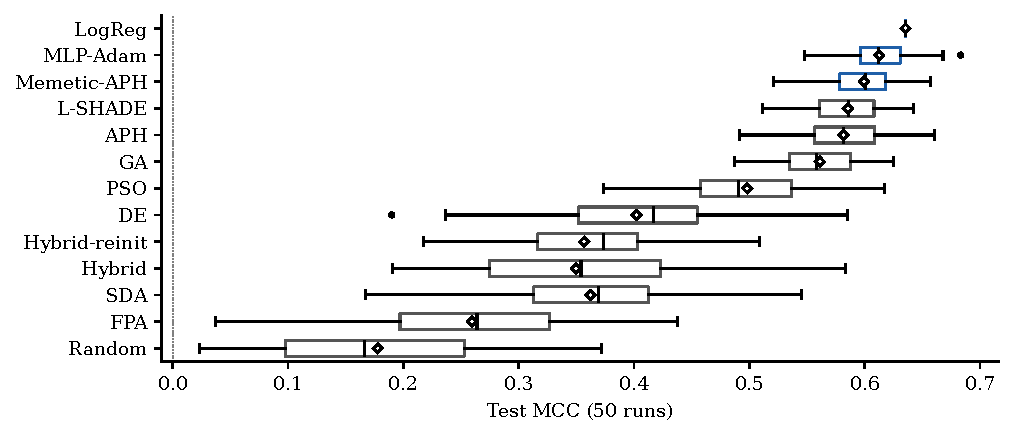
\includegraphics[width=\linewidth]{mcc_boxplots.pdf}
\caption{Test MCC over 50 runs on CNN features. Grey: gradient-free optimisers; blue: methods using gradients. Diamonds mark means.}
\label{fig:box}
\end{figure}

\begin{figure}[!t]
\centering
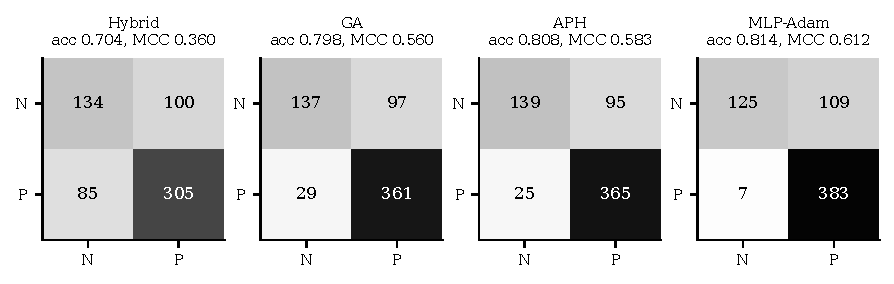
\includegraphics[width=\linewidth]{confusion.pdf}
\caption{Test confusion matrices (rows: true, columns: predicted; N = normal, P = pneumonia) of the median-MCC run of each method. Accuracy and MCC are computed from the displayed cells.}
\label{fig:confusion}
\end{figure}

\subsection{Statistical significance}\label{sec:stats}
The Friedman test rejects equal performance of the ten gradient-free optimisers ($\chi^2_F=\FriedmanChi$, $p=\FriedmanP$; Table~\ref{tab:friedman}). In the critical-difference diagram (Fig.~\ref{fig:cd}) the groups of methods that are not significantly different are \CDGroups; the two hybrids are thus separated from L-SHADE, APH, GA and PSO but not from DE, SDA or FPA. Pairwise tests on test MCC (Table~\ref{tab:wilcoxon}) show that the hybrid improves on FPA ($\bar\Delta=+0.090$, $\hat A=0.75$) and random search, is below PSO, GA and L-SHADE with large effects ($\hat A\le0.08$) and below DE with a medium effect ($\hat A=0.34$; not separated by the Nemenyi test), and does not differ from SDA or from its re-initialisation variant. SDA is better than FPA ($\bar\Delta=\SdaFpaDelta$).

Test MCC is, however, a noisy endpoint for comparing optimisers: it is evaluated at a fixed threshold on a test folder whose distribution differs from the training data. Tables~\ref{tab:endpoints} and \ref{tab:contrasts} therefore add the final training fitness and validation MCC. Three statements change. First, SDA reaches a lower training fitness than the hybrid in all 50 runs (median \FitSda{} against \FitHybrid) and a higher validation MCC (\ValSda{} against \ValHybrid): the hybrid is a worse optimiser than its second component, not an equivalent one. Second, the transfer variant reaches a lower fitness than the re-initialisation variant in all 50 runs, although their MCC values do not differ. Third, the hybrid reaches a lower training fitness than DE in \WinFitHybridde{} of 50 runs (median \FitHybrid{} against \FitDe) while DE has the higher validation and test MCC, so the ordering of these two depends on the endpoint. Lower training loss does not imply higher test MCC across methods.

Test-set sampling uncertainty is also substantial: the 95\% interval of a single model's MCC is about $\pm\OneModelLo$ to $\pm\OneModelHi$. For run-averaged differences (Table~\ref{tab:bootstrap}) the contrasts hybrid--FPA, L-SHADE--GA, APH--GA and logistic regression--L-SHADE remain resolved, whereas hybrid--SDA, APH--L-SHADE, MLP--APH and memetic APH--MLP are not. Restricting the test set to the \NoOverlapN{} images whose patient identifier does not occur in the training folder preserves the ranking of methods (Spearman $\rho=\NoOverlapRho$), and the sensitivity of logistic regression is the same on pneumonia images with and without an overlapping identifier (\LRSensOverlap\% and \LRSensOther\%), so there is no sign of memorised patients.

\begin{table}[!t]
\centering
\caption{Friedman test over the ten gradient-free optimisers (MCC, $N=50$ paired runs): $\chi^2_F=364.78$, $p=4.4\times 10^{-73}$. Mean ranks (1 = best) and Nemenyi critical difference $\mathrm{CD}_{0.05}=1.916$. Nemenyi $p$-values are given against the original hybrid and against APH.}
\label{tab:friedman}
\footnotesize
\resizebox{\linewidth}{!}{%
\begin{tabular}{lccc}
\toprule
Optimiser & Mean rank & $p$ vs Hybrid & $p$ vs APH \\
\midrule
L-SHADE & 1.80 & $<$0.001 & 1.000 \\
APH (redesigned hybrid) & 2.06 & $<$0.001 & -- \\
GA & 2.66 & $<$0.001 & 0.993 \\
PSO & 3.96 & $<$0.001 & 0.054 \\
DE & 5.89 & 0.831 & $<$0.001 \\
Hybrid FPA--SDA (re-init) & 6.78 & 1.000 & $<$0.001 \\
Hybrid FPA--SDA (transfer) & 6.88 & -- & $<$0.001 \\
SDA & 6.93 & 1.000 & $<$0.001 \\
FPA & 8.58 & 0.134 & $<$0.001 \\
Random search & 9.46 & $<$0.001 & $<$0.001 \\
\bottomrule
\end{tabular}}
\end{table}


\begin{figure}[!t]
\centering
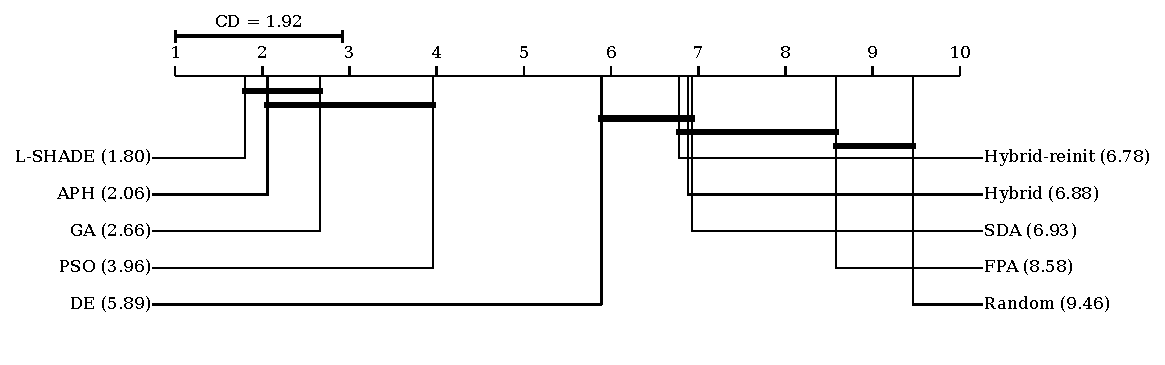
\includegraphics[width=\linewidth]{cd_diagram.pdf}
\caption{Critical-difference diagram (Nemenyi, $\alpha=0.05$, $N=50$) for test MCC. Methods joined by a bar are not significantly different; $\mathrm{CD}=\CDvalue$.}
\label{fig:cd}
\end{figure}

\begin{table}[!t]
\centering
\caption{Pairwise Wilcoxon signed-rank tests on MCC (50 paired runs), Holm-adjusted within each block. $\bar\Delta$: difference of means; $\tilde\Delta$: median of the 50 paired differences (first method minus second). $\hat A$: Vargha--Delaney effect size ($>0.5$ favours the first method; $|\hat A-0.5|\ge 0.21$ is large).}
\label{tab:wilcoxon}
\footnotesize
\resizebox{\linewidth}{!}{%
\begin{tabular}{llrrcc}
\toprule
Method & vs & $\bar\Delta$ & $\tilde\Delta$ & $p_{\mathrm{Holm}}$ & $\hat A$ \\
\midrule
Hybrid FPA--SDA (transfer) & FPA & +0.090 & +0.070 & $<$0.001 & 0.75 \\
 & SDA & -0.013 & -0.045 & 0.618 & 0.45 \\
 & Hybrid FPA--SDA (re-init) & -0.007 & +0.004 & 0.833 & 0.47 \\
 & Random search & +0.172 & +0.166 & $<$0.001 & 0.91 \\
 & PSO & -0.148 & -0.151 & $<$0.001 & 0.08 \\
 & DE & -0.052 & -0.061 & 0.012 & 0.34 \\
 & GA & -0.211 & -0.209 & $<$0.001 & 0.02 \\
 & L-SHADE & -0.236 & -0.229 & $<$0.001 & 0.01 \\
 & APH (redesigned hybrid) & -0.232 & -0.229 & $<$0.001 & 0.01 \\
\midrule
SDA & FPA & +0.103 & +0.103 & $<$0.001 & 0.81 \\
\midrule
APH (redesigned hybrid) & L-SHADE & -0.004 & -0.012 & 0.415 & 0.47 \\
 & GA & +0.020 & +0.025 & 0.004 & 0.65 \\
 & PSO & +0.083 & +0.091 & $<$0.001 & 0.88 \\
 & DE & +0.179 & +0.169 & $<$0.001 & 0.96 \\
\midrule
Hybrid + Adam (memetic) & Adam from random init. & +0.070 & +0.074 & $<$0.001 & 0.92 \\
 & MLP, backprop (Adam) & -0.034 & -0.035 & $<$0.001 & 0.15 \\
\bottomrule
\end{tabular}}
\end{table}


\begin{table}[!t]
\centering
\caption{Three endpoints for the gradient-free optimisers (50 paired runs): final training fitness (the quantity optimised; median), validation MCC and test MCC (means), with mean Friedman ranks (1 = best). Friedman tests: fitness $\chi^2_F=437.2$, validation MCC $\chi^2_F=405.2$, test MCC $\chi^2_F=364.8$ (all $p<10^{-40}$).}
\label{tab:endpoints}
\footnotesize
\resizebox{\linewidth}{!}{%
\begin{tabular}{lcccccc}
\toprule
 & \multicolumn{2}{c}{Training fitness} & \multicolumn{2}{c}{Validation MCC} & \multicolumn{2}{c}{Test MCC} \\
Optimiser & median & rank & mean & rank & mean & rank \\
\midrule
L-SHADE & 0.159 & 1.26 & 0.797 & 1.44 & 0.585 & 1.80 \\
APH (redesigned hybrid) & 0.176 & 1.90 & 0.784 & 1.98 & 0.581 & 2.06 \\
GA & 0.240 & 3.16 & 0.761 & 2.74 & 0.561 & 2.66 \\
PSO & 0.276 & 3.76 & 0.708 & 3.90 & 0.498 & 3.96 \\
SDA & 0.455 & 4.96 & 0.548 & 6.34 & 0.362 & 6.93 \\
Hybrid FPA--SDA (transfer) & 0.701 & 6.34 & 0.516 & 7.06 & 0.350 & 6.88 \\
DE & 0.819 & 6.66 & 0.574 & 5.96 & 0.402 & 5.89 \\
Hybrid FPA--SDA (re-init) & 1.725 & 7.96 & 0.520 & 6.88 & 0.357 & 6.78 \\
FPA & 4.905 & 9.10 & 0.376 & 8.94 & 0.260 & 8.58 \\
Random search & 6.341 & 9.90 & 0.275 & 9.76 & 0.178 & 9.46 \\
\bottomrule
\end{tabular}}
\end{table}


\begin{table}[!t]
\centering
\caption{Key contrasts on the three endpoints (50 paired runs). ``Wins'': number of runs in which the first method is better (lower fitness, higher MCC). $p$: Wilcoxon signed-rank, Holm-adjusted over the seven contrasts of each endpoint.}
\label{tab:contrasts}
\footnotesize
\resizebox{\linewidth}{!}{%
\begin{tabular}{llcccccc}
\toprule
 & & \multicolumn{2}{c}{Training fitness} & \multicolumn{2}{c}{Validation MCC} & \multicolumn{2}{c}{Test MCC} \\
Method & vs & wins & $p$ & wins & $p$ & wins & $p$ \\
\midrule
Hybrid FPA--SDA (transfer) & SDA & 0/50 & $<$0.001 & 15/50 & 0.028 & 22/50 & 0.927 \\
Hybrid FPA--SDA (transfer) & Hybrid FPA--SDA (re-init) & 50/50 & $<$0.001 & 25/50 & 0.916 & 26/50 & 0.927 \\
Hybrid FPA--SDA (transfer) & DE & 32/50 & 0.003 & 12/50 & $<$0.001 & 15/50 & 0.016 \\
Hybrid FPA--SDA (transfer) & FPA & 50/50 & $<$0.001 & 47/50 & $<$0.001 & 43/50 & $<$0.001 \\
SDA & FPA & 50/50 & $<$0.001 & 46/50 & $<$0.001 & 36/50 & $<$0.001 \\
APH (redesigned hybrid) & L-SHADE & 11/50 & $<$0.001 & 16/50 & 0.012 & 19/50 & 0.927 \\
APH (redesigned hybrid) & GA & 44/50 & $<$0.001 & 37/50 & $<$0.001 & 37/50 & 0.011 \\
\bottomrule
\end{tabular}}
\end{table}


\begin{table}[!t]
\centering
\caption{Uncertainty due to the fixed 624-image test set. For each contrast, test images are resampled with replacement (2,000 bootstrap samples) and the difference in run-averaged MCC is recomputed from the stored predictions; seeds are held fixed. Intervals that include 0 indicate contrasts not resolved by this test set, even when they are significant across seeds (Table~\ref{tab:wilcoxon}).}
\label{tab:bootstrap}
\footnotesize
\resizebox{\linewidth}{!}{%
\begin{tabular}{llrc}
\toprule
Method & vs & $\bar\Delta$ MCC & 95\% CI (test images) \\
\midrule
APH (redesigned hybrid) & GA & +0.020 & [+0.008, +0.032] \\
APH (redesigned hybrid) & L-SHADE & -0.004 & [-0.014, +0.006] \\
L-SHADE & GA & +0.024 & [+0.012, +0.037] \\
Hybrid FPA--SDA (transfer) & SDA & -0.013 & [-0.029, +0.002] \\
Hybrid FPA--SDA (transfer) & FPA & +0.090 & [+0.072, +0.106] \\
Logistic regression & L-SHADE & +0.050 & [+0.004, +0.094] \\
MLP, backprop (Adam) & APH (redesigned hybrid) & +0.031 & [-0.005, +0.068] \\
APH + Adam (memetic) & MLP, backprop (Adam) & -0.013 & [-0.031, +0.005] \\
\bottomrule
\end{tabular}}
\end{table}


\subsection{Transition point}
Table~\ref{tab:tau} and Fig.~\ref{fig:tau} vary $\tau$ while keeping $T=150$; SDA alone ($\tau=0$) and FPA alone ($\tau=150$) are included with the same seeds. Mean MCC falls from 0.381 (SDA alone) and 0.380 ($\tau=25$) to 0.235 ($\tau=125$) and 0.243 (FPA alone). Page's test confirms a decreasing trend ($L=\PageL$, $p=\PageP$), but no pair of adjacent settings differs significantly (smallest $p_{\mathrm{Holm}}=\TauAdjMin$) and none of the 20 individual runs decreases monotonically. The value $\tau=75$ used in our original draft is not an optimum, and no hybrid schedule improves on SDA alone.

\begin{table}[!t]
\centering
\caption{Sensitivity of the hybrid to the transition iteration $\tau$ (20 paired runs; $\tau=0$ is SDA alone and $\tau=150$ FPA alone, same seeds). Friedman over $\tau\in\{25,\dots,125\}$: $\chi^2_F=29.52$, $p=6.1\times 10^{-6}$. Page's trend test over all seven settings: $L=2591$, $p=3.3\times 10^{-12}$. $p_{\mathrm{Holm}}$: Wilcoxon against $\tau=75$.}
\label{tab:tau}
\footnotesize
\resizebox{\linewidth}{!}{%
\begin{tabular}{lccccccc}
\toprule
$\tau$ & 0 & 25 & 50 & 75 & 100 & 125 & 150 \\
\midrule
Accuracy (\%) & 71.56 & 71.62 & 70.77 & 70.03 & 66.82 & 64.29 & 63.99 \\
MCC & 0.381 & 0.380 & 0.356 & 0.345 & 0.286 & 0.235 & 0.243 \\
AUC & 0.774 & 0.771 & 0.765 & 0.746 & 0.710 & 0.684 & 0.675 \\
$p_{\mathrm{Holm}}$ (MCC) & 0.568 & 0.131 & 0.568 & -- & 0.568 & 0.002 & $<$0.001 \\
\bottomrule
\end{tabular}}
\end{table}


\begin{figure}[!t]
\centering
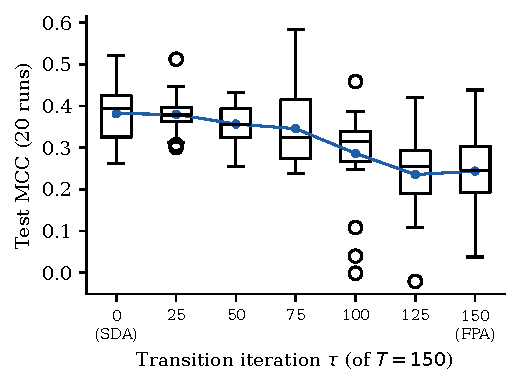
\includegraphics[width=0.62\linewidth]{tau_study.pdf}
\caption{Test MCC of the hybrid as a function of the transition iteration $\tau$ (20 runs each; line: means).}
\label{fig:tau}
\end{figure}

\subsection{Redesign and ablation}\label{sec:redesign}
APH raises the hybrid's test MCC from \MCCHybrid{} to \MCCAph{} ($\bar\Delta=+0.232$, $\hat A=0.99$) and is ahead of GA on all three endpoints (Table~\ref{tab:contrasts}), PSO and DE. Compared with L-SHADE, which uses the same framework without the plant-inspired operators, test MCC does not differ ($p_{\mathrm{Holm}}=0.42$), but APH reaches a lower training fitness in only \WinFitAphlShade{} of 50 runs (median \FitAph{} against \FitLshade) and a lower validation MCC (\ValAph{} against \ValLshade): adding the FPA and SDA operators to L-SHADE slightly worsens optimisation on this task. APH is an instance of adaptive strategy selection in DE \citep{qin2009sade,gong2011strategy} with four extra operators and is not proposed as a new algorithm.

The ablation (Table~\ref{tab:ablation}) locates the source of APH's advantage over the original hybrid. Removing binomial crossover and replacing adaptive operator selection by uniform probabilities cost about the same (\AblNoCx{} and \AblUniform; the two variants do not differ, $p=\AblUniformVsNoCx$), and both intervals exclude zero on the test-image bootstrap. Removing the current-to-$p$best operator---leaving only the FPA and SDA operators, with all adaptation mechanisms intact---costs far more (\AblPlant) and returns MCC to 0.382, the level of the original hybrid. The operator-selection mechanism allocates \ShareAnimal\% of all trials to that operator, against \ShareLocal\% (FPA local), \ShareGravity\% (SDA gravity) and \ShareGlobal\% (FPA global). The contributions of SHADE parameter adaptation and population-size reduction were not ablated. As stated in Section~\ref{sec:protocol}, these comparisons are exploratory. The cross-field methods OpenAI-ES and ZO-SGD reach MCC 0.40 and 0.39 at this budget.

\begin{table}[!t]
\centering
\caption{Component ablation of APH and cross-field gradient-free baselines (20 paired runs). $\bar\Delta$: mean MCC of the variant minus APH; CI: 95\% test-image bootstrap interval of $\bar\Delta$; $p_{\mathrm{Holm}}$: Wilcoxon signed-rank test against APH across runs.}
\label{tab:ablation}
\footnotesize
\resizebox{\linewidth}{!}{%
\begin{tabular}{lccrcc}
\toprule
Variant & MCC & AUC & $\bar\Delta$ & CI & $p_{\mathrm{Holm}}$ \\
\midrule
APH (full) & 0.581 & 0.899 & -- & -- & -- \\
-- adaptive operator selection (uniform) & 0.552 & 0.883 & -0.029 & [-0.045, -0.012] & 0.165 \\
-- binomial crossover (full-vector moves) & 0.550 & 0.875 & -0.031 & [-0.048, -0.013] & 0.028 \\
-- current-to-$p$best operator (plant operators only) & 0.382 & 0.774 & -0.199 & [-0.226, -0.172] & $<$0.001 \\
\midrule
L-SHADE & 0.587 & 0.900 & +0.006 & [-0.009, +0.021] & 0.622 \\
OpenAI-ES & 0.402 & 0.779 & -0.180 & [-0.203, -0.155] & $<$0.001 \\
ZO-SGD (SPSA) & 0.386 & 0.770 & -0.195 & [-0.219, -0.170] & $<$0.001 \\
\bottomrule
\end{tabular}}
\end{table}


\subsection{Memetic variants and convergence}
Using the hybrid as an initialiser for Adam (memetic) improves on Adam started from the best of the same random population (\MCCMemeticHybrid{} vs \MCCAdamOnly, $\hat A=0.92$), and APH+Adam reaches \MCCMemeticAph. Neither surpasses the MLP trained by standard backpropagation with standard initialisation (\MCCMlpAdam; Table~\ref{tab:wilcoxon}). The benefit of the metaheuristic phase is therefore relative to a poor uniform initialisation in $[-1,1]^D$ rather than to gradient training as normally practised. Fig.~\ref{fig:conv} shows that the hybrid's fitness remains above that of GA, L-SHADE and APH throughout. The transition at $\tau=75$ is followed by a marked acceleration: the median log-fitness decreases by \SlopePre{} per iteration over iterations 50--75 and by \SlopePost{} over iterations 75--100 (\SlopeRatio$\times$), consistent with the SDA phase driving most of the progress. Per-run times are 36--60\,s for all gradient-free optimisers, against about 1\,s for the gradient-trained MLP.

\begin{figure}[!t]
\centering
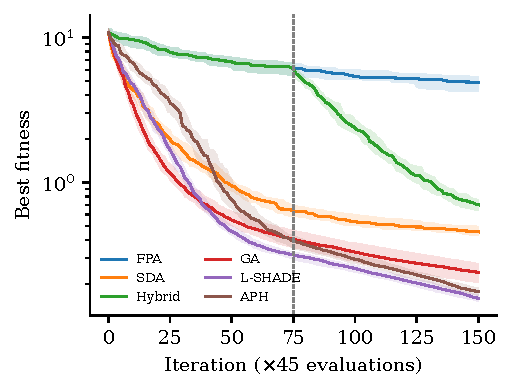
\includegraphics[width=0.62\linewidth]{convergence.pdf}
\caption{Best-so-far fitness (median and inter-quartile range over 50 runs); dashed line: $\tau=75$.}
\label{fig:conv}
\end{figure}

\subsection{Fine-tuned features and cross-validation}\label{sec:finetune}
Table~\ref{tab:finetune} reports end-to-end fine-tuning. On the official split, accuracy on the test folder is \FTOffAcc\% (\FTOffMin--\FTOffMax\% over five seeds), against \ACCLogreg\% for the best classifier on frozen features; specificity is \FTOffSpec\%, while accuracy on the validation subset is \FTValAcc\%. Under patient-grouped cross-validation, pooled out-of-fold accuracy is \FTCvAcc\% with a specificity of \FTCvSpec\%. Out-of-fold accuracy is \FTCvAccTrainFolder\% for images from the official training folder and \FTCvAccTestFolder\% for images from the official test folder: the test folder is harder even when its images take part in training, which confirms a distribution difference between the two folders. The two protocols answer different questions, and the cross-validated figure must not be compared with results reported on the official test folder.

\begin{table}[!t]
\centering
\caption{End-to-end fine-tuning of ResNet-50 by backpropagation (mean$\pm$SD over seeds). Official split: trained on the optimisation subset, epoch chosen on the validation subset, evaluated once on the official test folder (5 seeds). Cross-validation: patient-grouped 5-fold over all 5,856 images, pooled out-of-fold predictions (3 seeds).}
\label{tab:finetune}
\footnotesize
\resizebox{\linewidth}{!}{%
\begin{tabular}{lccccc}
\toprule
Protocol & Acc. (\%) & Sens. (\%) & Spec. (\%) & MCC & AUC \\
\midrule
Official test folder (624 images) & 89.04$\pm$1.25 & 99.23$\pm$0.31 & 72.05$\pm$3.75 & 0.773$\pm$0.024 & 0.974$\pm$0.005 \\
5-fold cross-validation (5,856 images) & 97.43$\pm$0.25 & 97.82$\pm$0.15 & 96.38$\pm$0.69 & 0.935$\pm$0.006 & 0.996$\pm$0.001 \\
\bottomrule
\end{tabular}}
\end{table}


Table~\ref{tab:cvhead} reports the 2048--16--2 head trained by each optimiser on the fine-tuned features inside the cross-validation. All methods lie between \CvHeadMin\% and \CvHeadMax\% accuracy. The original hybrid reaches \CvHeadHybrid\% in the Glorot-scaled space and \CvHeadHybridBox\% in the $[-1,1]$ box, against \CvHeadLshade\% for L-SHADE, \CvHeadMlp\% for the backpropagation-trained MLP and \CvHeadLogreg\% for logistic regression. With a representation in which the classes are almost linearly separable, the differences between optimisers that dominate the frozen-feature benchmark shrink to about one percentage point. They remain systematic: across the 50 fold--run pairs the hybrid is below GA, L-SHADE and the gradient-trained classifiers and above FPA ($p_{\mathrm{Holm}}\le0.001$), and it does not differ from SDA (Friedman over the six gradient-free variants $p=\CvHeadFriedmanP$).

\begin{table}[!t]
\centering
\caption{Classifier head trained by each optimiser on fine-tuned features inside the cross-validation (5 folds $\times$ 10 runs; mean$\pm$SD over the 50 fold--run pairs). Gradient-free optimisers search the Glorot-scaled space unless stated. $p_{\mathrm{Holm}}$: Wilcoxon signed-rank test against the hybrid on MCC.}
\label{tab:cvhead}
\footnotesize
\resizebox{\linewidth}{!}{%
\begin{tabular}{lcccc}
\toprule
Method & Acc. (\%) & Spec. (\%) & MCC & $p_{\mathrm{Holm}}$ \\
\midrule
Logistic regression & 97.63$\pm$0.42 & 95.58$\pm$1.17 & 0.940$\pm$0.011 & $<$0.001 \\
MLP, backprop (Adam) & 97.49$\pm$0.43 & 95.65$\pm$1.16 & 0.937$\pm$0.011 & $<$0.001 \\
GA & 97.40$\pm$0.49 & 95.28$\pm$1.45 & 0.934$\pm$0.013 & $<$0.001 \\
L-SHADE & 97.36$\pm$0.44 & 95.22$\pm$1.28 & 0.933$\pm$0.011 & $<$0.001 \\
SDA & 97.10$\pm$0.48 & 95.89$\pm$1.09 & 0.927$\pm$0.012 & 0.931 \\
Hybrid FPA--SDA & 97.08$\pm$0.50 & 95.87$\pm$1.25 & 0.927$\pm$0.012 & -- \\
FPA & 96.85$\pm$0.58 & 95.49$\pm$1.60 & 0.921$\pm$0.014 & 0.001 \\
Hybrid FPA--SDA, $[-1,1]$ box & 96.83$\pm$0.56 & 95.31$\pm$1.39 & 0.920$\pm$0.014 & 0.001 \\
\bottomrule
\end{tabular}}
\end{table}


%% ===========================================================================
\section{Discussion}\label{sec:discussion}

\paragraph{Why the sequential hybrid does not help} With $\gamma=1$, FPA's global operator and SDA's wind operator are the same Lévy move, so FPA and SDA differ only in their remaining operators (FPA's differential local move versus SDA's animal and gravity dispersal) and in how often the Lévy move is used. SDA outperforms FPA, the hybrid's fitness improves much faster once the SDA phase starts, and no hybrid schedule improves on SDA alone; the hybrid therefore inherits the performance of its second phase. We did not ablate SDA's individual operators, so which of them is responsible remains open. A further factor is that all FPA and SDA operators perturb every coordinate; in APH, however, removing crossover reduced MCC by only about 0.03, so partial moves explain a small part of the gap. The decisive component in our ablation is the current-to-$p$best direction. The search box $[-1,1]^D$, inherited from the original implementation, is much wider than standard weight initialisations; its effect on the frozen-feature benchmark was not tested.

\paragraph{Relation to the metaphor debate} Our redesign followed the usual path of improving a hybrid by adding adaptive mechanisms, and it produced a method that appears better than GA and PSO. Without the ablation, it would have been easy to present APH as a new, superior plant-inspired algorithm. The analysis shows instead that APH optimises slightly worse than L-SHADE and that it owes its advantage over the original hybrid to a DE operator; its plant-inspired operators, although selected in \SharePlant\% of trials, bring no benefit on this task, illustrating at the component level the concern raised by \citet{sorensen2015metaphor} and \citet{camacho2023exposing}. We recommend that hybrid metaheuristics proposed for neural-network training be accompanied by (i) equal-budget comparisons with L-SHADE or CMA-type baselines, (ii) operator-removal ablations and (iii) paired statistics.

\paragraph{Representation versus optimiser} At equal or lower cost, gradient-based training produced the best classifiers on frozen features: logistic regression reached 82.7\% accuracy and the MLP an AUC of 0.937 in about one second, compared with 36--60\,s for gradient-free optimisers. Fine-tuning the network, which is itself gradient training, moved accuracy much further than any change of optimiser, and on the fine-tuned features the original hybrid is within about one percentage point of every other method (Section~\ref{sec:finetune}). For this application the useful question is therefore how to obtain a good representation, not which metaheuristic trains the last layers. On frozen features the stronger methods show high sensitivity but modest specificity (at most about 60\%) on the test folder, while specificity on the validation subset is much higher (\LRValSpec\% for logistic regression); together with the cross-validation result this points to a distribution difference between the official folders, and threshold calibration and external validation would be required before any clinical use. Gradient-free training remains defensible where gradients are genuinely unavailable---non-differentiable objectives, quantised or hardware-in-the-loop models---and these settings, not standard supervised training, are where plant-inspired operators would need to be evaluated.

\paragraph{Limitations} The study uses one dataset and one network architecture, so its conclusions are limited to this task; the budget is fixed at 6,795 evaluations (about 0.2 evaluations per dimension on the CNN head) within a $[-1,1]$ search box; competitor parameters are standard defaults rather than individually tuned; all comparisons use one fixed test set, whose sampling uncertainty is reported but not reduced; APH and the memetic variants were designed after the benchmark results were known and have not been confirmed on fresh seeds; SHADE parameter adaptation and population-size reduction were not ablated; patient overlap between the official training and test folders cannot be fully excluded; the step-size parameter $\gamma=1$ and the search box of the frozen-feature benchmark were inherited from the original implementation and not varied; the head-training experiments on fine-tuned features use the features of one seed per fold; the cross-validation relies on patient identifiers parsed from file names; and the SDA operators could not be traced to a verifiable primary source, so we evaluate them as implemented.

%% ===========================================================================
\section{Conclusions}\label{sec:conclusion}
On this task and under a controlled protocol, the sequential FPA--SDA hybrid was a worse optimiser than its SDA component, was below GA, PSO and L-SHADE on every endpoint, and was below gradient-trained classifiers on frozen CNN features; on the original 138,530-dimensional pipeline with standardised inputs none of the gradient-free optimisers tested exceeded chance level. A redesigned hybrid with adaptive operator selection and success-history adaptation approached L-SHADE, but owed this to a differential-evolution operator, and adding the plant-inspired operators to L-SHADE slightly worsened optimisation. Fine-tuning the network raised accuracy to \FTOffAcc\% on the official test folder and \FTCvAcc\% under patient-grouped cross-validation, and on fine-tuned features all optimisers, including the original hybrid, were within about one percentage point. Whether these findings extend to other datasets, budgets and published variants of FPA remains to be tested; we recommend that hybrids of this kind be reported with equal-budget baselines, component ablations and the training objective as an endpoint.

%% ===========================================================================
\section*{Data and code availability}
The dataset is publicly available \citep{kaggle2018cxr,kermany2018}. Code, configurations, per-run outputs (including test-set probabilities) and the script that generates every table and figure are available at \citet{alsbakhi2026code}; the data used are the Kaggle redistribution of the dataset released by \citet{kermany2018}. \emph{An archived release with a DOI must be added here before submission.}

\section*{CRediT authorship contribution statement}
\textbf{Mona Alsbakhi:} Conceptualization, Methodology, Software, Investigation, Writing -- original draft. \textbf{Mohammed Lubbad:} Methodology, Validation, Writing -- review \& editing. \textbf{Mohammed Alhanjouri:} Supervision, Writing -- review \& editing.

\section*{Declaration of competing interest}
The authors declare that they have no known competing financial interests or personal relationships that could have appeared to influence the work reported in this paper.

\section*{Funding}
This research did not receive any specific grant from funding agencies in the public, commercial, or not-for-profit sectors.

\section*{Ethics statement}
This study used a public, de-identified dataset; no ethical approval or informed consent was required.

\section*{Declaration of generative AI and AI-assisted technologies in the manuscript preparation process}
During the preparation of this work the authors used Claude (Anthropic) to re-implement the optimisation pipeline, run and analyse the experiments, check references and draft and revise the text of the manuscript. The authors reviewed and edited the content as needed and take full responsibility for the content of the published article.

\appendix
\section{Parameter settings}\label{app:params}
\begin{table}[H]
\centering
\caption{Parameter settings. Common to all gradient-free methods: population/batch $n=45$, $T=150$ iterations (budget $6{,}795$ evaluations), box $[-1,1]^D$, uniform initialisation, one shared seed per run. ``Sel.'': replacement rule ($<$ strictly better; $\le$ not worse).}
\label{tab:params}
\footnotesize
\begin{tabular}{p{2.6cm}p{8.6cm}c}
\toprule
Method & Parameters & Sel. \\
\midrule
FPA & $p=0.8$, $\gamma=1$, Lévy $\beta=1.5$ (Mantegna) & $<$ \\
SDA & $(P_{\mathrm{wind}},P_{\mathrm{animal}},P_{\mathrm{gravity}})=(0.70,0.15,0.15)$, gravity step $U(-0.1,0.1)$, $\beta=1.5$ & $<$ \\
Hybrid FPA--SDA & FPA then SDA, $\tau=75$; transfer or re-initialisation ($\sigma_{\mathrm{init}}=0.1$) & $<$ \\
Random search & uniform resampling, per-slot replacement & $<$ \\
PSO & $w=0.7298$, $c_1=c_2=1.49618$, $v_{\max}=0.2(ub-lb)$ & $<$ \\
GA & steady state, binary tournament, BLX-$\alpha$ ($\alpha=0.5$), Gaussian mutation (rate $10/D$, $\sigma=0.2$), replaces worst & $<$ \\
DE/rand/1/bin & $F=0.5$, $CR=0.9$ & $\le$ \\
L-SHADE & current-to-$p$best/1/bin, $p=0.11$, memory $H=6$, archive size = population, population $45\to4$ & $\le$ \\
APH & as L-SHADE; four operators (O1--O4), probability matching (rate $0.3$, floor $0.05$), Lévy clipped to $\pm3$ & $\le$ \\
OpenAI-ES & 22 antithetic pairs per iteration, $\sigma=0.02$, Adam step $0.01$, centred ranks; starts from best of 45 uniform samples & -- \\
ZO-SGD & two-point SPSA, $\epsilon=10^{-3}$, step $10^{-3}$; starts from best of 45 uniform samples & -- \\
Memetic variants & inner optimiser for 75 iterations (hybrid with $\tau=37$, or APH), then 300 full-batch Adam steps, learning rate $10^{-3}$ & -- \\
MLP, backprop & scikit-learn \texttt{MLPClassifier}, same hidden layers, Adam ($10^{-3}$) or SGD ($10^{-3}$, momentum $0.9$), $L_2=10^{-3}$, batch 64, $\le150$ epochs, early stopping on a random 10\% split (patience 15), no class weights & -- \\
Logistic regression & $C=1$, balanced class weights & -- \\
\bottomrule
\end{tabular}
\end{table}


\bibliographystyle{elsarticle-harv}
\bibliography{refs}

\end{document}
